\newsection
\subsection{Interaction}
\label{sec:interaction}
\sectionauthors{Joon Sung Park, Chris Donahue, Mina Lee, Siddharth Karamcheti, Dorsa Sadigh, Michael S. Bernstein}

\begin{figure}[!ht]
\centering
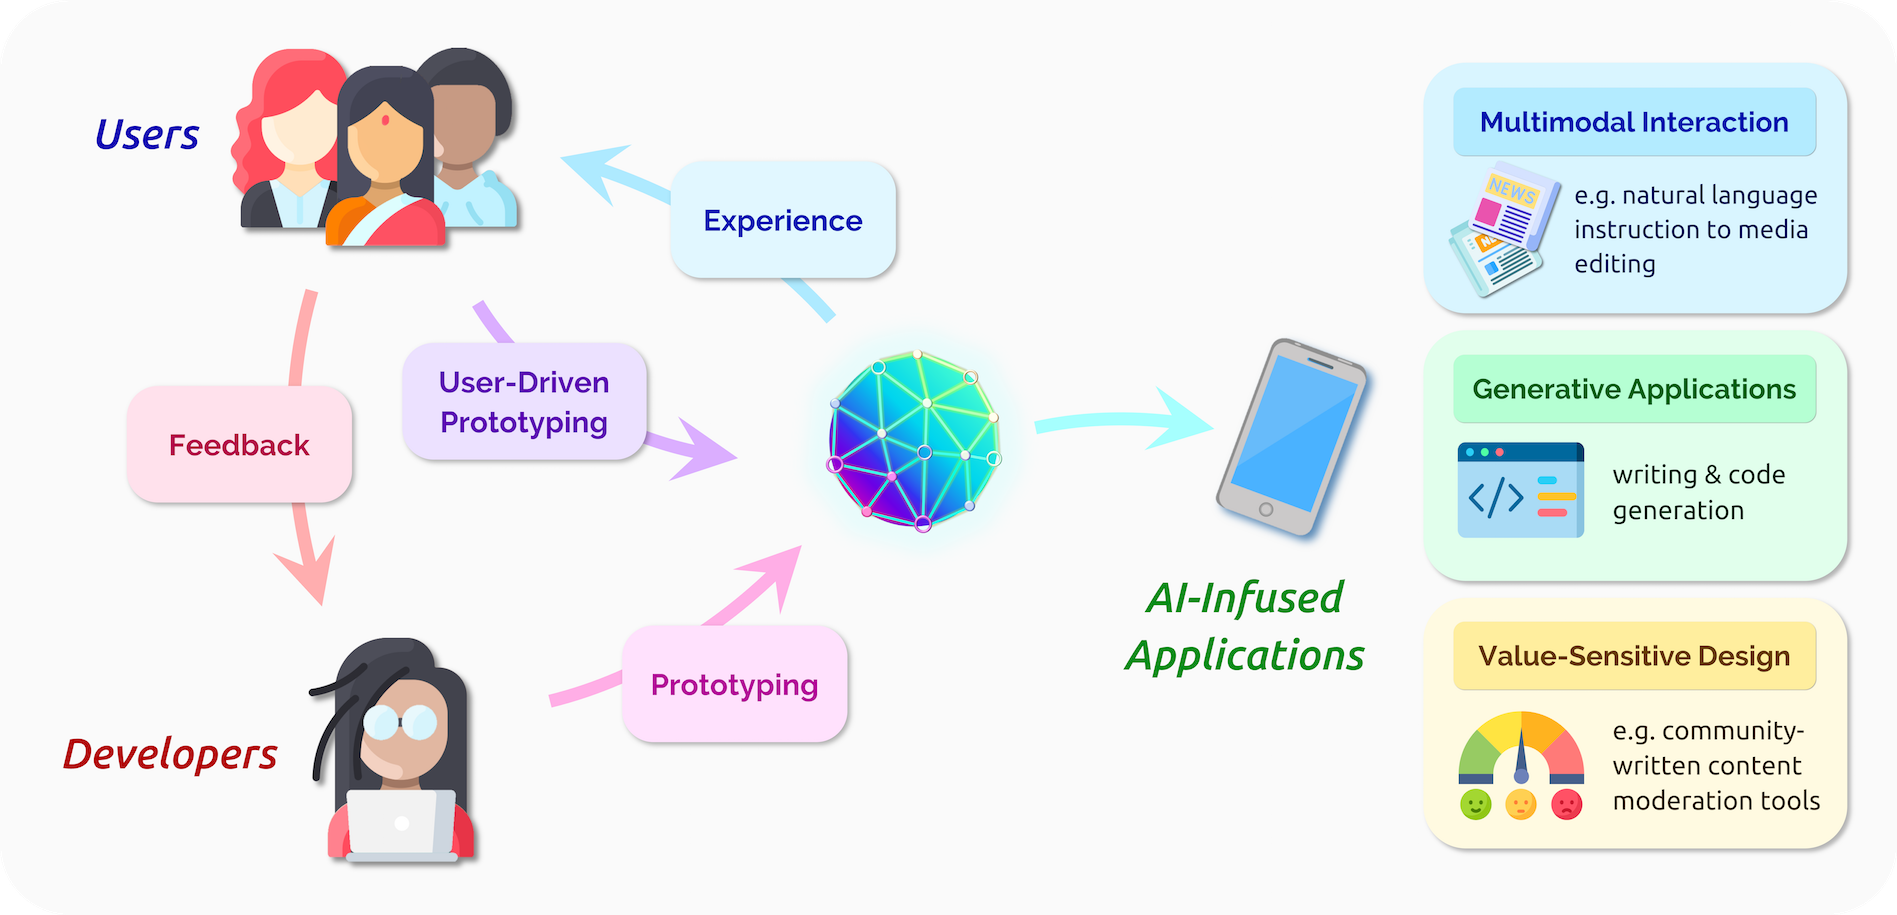
\includegraphics[width=\linewidth]{capabilities/figures/Interaction.png}
\caption{\label{fig:interaction} Foundation models will bring significant opportunities to developers by lowering the difficulty threshold for building AI-infused applications, and to the application users by raising the ceiling for what types of interactions are achievable. In some cases, the line between developers and users will start to blur, and users may be able to easily develop their own AI applications, for instance with natural language.}
\end{figure}

The early forms of foundation models such as GPT-3~\citep{brown2020gpt3} and DALL·E~\citep{ramesh2021zeroshot} have demonstrated a high level of versatility both in terms of their ability to let even non-ML experts to prototype powerful AI-infused applications, and their ability to seamlessly integrate modalities ranging from texts to images. As the development of foundation models matures, the models' capacity will continue to expand and their versatility may ultimately lead to fundamental changes in how we interact with AI by allowing us to rapidly prototype and build highly dynamic and generative AI-infused applications. In this section, we discuss the opportunities that these changes present from the perspectives of two important stakeholders: (1)~applications developers who will interact with foundation models to design user experience, and (2)~end-users who will use or be affected by the AI-infused applications powered by foundation models. Finally, we consider scenarios in which the line that rigidly separates developers and end-users today may start to blur, affording new opportunities for creating AI-infused applications that more closely satisfy users' needs and values.

\subsubsection{Impact on AI-infused application developers' development process} 
How will foundation models transform the way developers create AI-infused applications? Despite the monumental progress in machine learning algorithms and systems infrastructure, some point out that designing novel and positive forms of human-AI interaction remains  difficult~\citep{Dove2017uxdesign, Cooper2014face}. The vast amount of data, computing resources, and skills needed to create a powerful task-specific model is frequently in conflict with the iterative prototyping process necessary to elicit and satisfy users' needs and values~\citep{Yang2016wireframing}. This challenge is further compounded by the fact that AI responses can be unpredictable, and models can produce a vast generative output space, making it difficult for people to build effective mental models of their performance. There has already been some progress on tackling these challenges in the form of work on interactive machine learning (\eg Crayon~\citep{Fails2003design}, Regroup~\citep{Amershi2012regroup}) and design frameworks for conveying uncertainty in AI to end-users (\eg principles of mixed-initiative~\citep{Horvitz1999mixedinit}). However, more work is still needed to overcome these obstacles~\citep{yang2020aiexamine}.

Foundation models pose important opportunities to address many of the challenges mentioned above. For instance, language-based foundation models' ability to take natural language as input, and to generalize to many downstream tasks, could significantly lower the difficulty ``threshold''~\citep{Myers2000ui} for application development, \ie~by enabling the development of sophisticated models without having to collect significant amounts of data and train large models from scratch. This could enable even non-ML experts to quickly prototype AI-infused applications. 
At the same time, the powerful generative and potentially multi-modal capabilities of foundation models could offer a far higher ``ceiling''~\citep{Myers2000ui} of what types of interactions are achievable both in terms of their quality and diversity as we will discuss below. However, how successfully we can leverage these capacities will depend on how effectively we can wrangle foundation models into forms that will be more manageable by application developers.

Unfortunately, the same generalizability and high ceiling that give foundation models their edge can also make these models difficult to work with, as they may be even more unpredictable and complex than single-purpose AI models. Indeed, recent work has shown that it can be difficult to make models like GPT-3 consistently perform the intended task~\citep{Reynolds2021prompt}, while understanding what it is capable of is still an active area of research~\citep{Hendrycks2020Measuring}. In an effort to improve the reliability and trustworthiness of AI-infused applications, we recommend that future work should continue to investigate how to achieve more predictable and robust behaviors from foundation models (\eg through fine-tuning, or in cases where the main mode of interaction is natural language prompt, through prompt-engineering~\citep{Reynolds2021prompt, Liu2021incontext}, calibrating~\citep{Zhao2021calibrate}, or pre-formatting a task-specific endpoint.\footnote{https://beta.openai.com/docs/guides/classifications} Please see \refsec{robustness} for more details). 

\subsubsection{Impact on end-user interaction with AI-infused applications} 
\label{sec:interaction-userimpact}
Beyond the new ways developers might create AI-infused applications, what changes will foundation models bring to the experience for end-users interacting with these applications? Existing design frameworks for developing user-facing AI applications focus on augmenting (rather than replacing) users' abilities as described by Douglas Engelbart~\citep{Engelbart1963augment}\dash{}we expect that these frameworks should and will remain relevant for the development of future AI-infused applications. For instance, maintaining users' agency and reflecting their values will continue to be a central theme for foundation model-powered applications. Additionally, the benefits of allowing AI agents to take initiatives and automate users' routines versus the benefits of waiting for users' direct manipulation~\citep{Shneiderman1997direct} will need to be carefully weighed~\citep{Horvitz1999mixedinit}. Moreover, users' values should be directly gathered and reflected through processes such as participatory~\citep{Lee2019} and value-sensitive design~\citep{smith2020keeping} that advocate for actively involving all stakeholders during the designing of the AI-infused applications. 

These issues may become especially salient with foundation models because the model may behave in ways that surprise and disappoint users and communities. Generative capabilities might expose biases or points of view that are counter to the communities' goals, or more insidiously, draw on such associations in their behavior without the community being aware. This will place a large burden on the groups utilizing foundation models to monitor their models' behavior, and to the extent possible, adapt them to act in appropriate ways.

While the design frameworks for thinking about AI-infused applications to augment users' abilities should remain the same, the actual forms of interactions that are attainable may dramatically diversify due to foundation models' powerful generative and multi-modal capacities. Already, early generations of what can be considered foundation model-powered software tools for multimedia creation and editing have started to drive a new frontier that empowers even novice content creators to generate high-quality multimedia from coarse, intuitive specifications (\eg paraphrasing for writers,\footnote{https://www.wordtune.com/} foreground segmentation for photographers,\footnote{https://helpx.adobe.com/photoshop/using/select-mask.html} mastering for musicians,\footnote{https://www.landr.com/} and code completion for programmers).\footnote{https://copilot.github.com/} Improved foundation models might enable even more ambitious tools (\eg a fan might provide thematic material for a song which will then be generated in the style of their favorite band, or a business owner might provide simple descriptions of their product which will be used to create a full website). Moreover, foundation models will be used to enrich static multimedia (\eg automatically remastering legacy multimedia content into new formats, or generating unique experiences for each player in new video games) and may even lead to new forms of multi-modal interactions using interfaces that themselves mix different modalities, such as visual and gesture-based interaction. 

We are starting to see glimpses of how foundation models might materialize into concrete interactions in applications ranging from AI Dungeon\footnote{https://play.aidungeon.io/main/home} to Microsoft PowerApps\footnote{https://powerapps.microsoft.com/en-us/} and CoPilot.\footnote{https://copilot.github.com/} As we start to envision new forms of interactions, it is of increasing importance for us to think critically about the potential implications these interactions will have on individual users and society to maximize their positive impact. For example, how will foundation model-powered applications change the way we communicate with one another? Will a powerful model write emails in our stead and if so, how will this reshape people's trust, credibility, and identity knowing that the writers may not have written the emails themselves, and how will this alter our writing styles~\citep{Hancock2020AI}? Who will own the authorship of the model-generated content and how could the shifting responsibilities and ownership of the consent be misused~\citep{Weiner2018} (see \refsec{economics} for a more in-depth discussion)? What are the long-term implications that foundation models will have on our work, language and culture~\citep{Hancock2020AI, Buschek2021writing}? Of particular relevance to this last question is the fact that foundation models are trained on observed data and do not necessarily inform us about causality. Hence, how can we ensure that the use of foundation models leads us to a desired future and not a repetition of the past? Though these issues are not necessarily unique to foundation models, they will be amplified and become more prevalent as foundation models accelerate the creation of effective AI-infused applications. 

\subsubsection{Blurring the line between developers and end-users}
\label{sec:interaction-blurring}
Today, the line that separates the developers of AI models and end-users is rigid\dash{}it is rarely the case that an end-user has the data, computing resources, and expertise to be able to develop a new model that suits one's values and needs well. While a generic model (\ie~one that is not specific to a specific user or community) could be sufficient in some cases, recent years have seen an increasing number of scenarios in which such models fail to serve users. For instance, a text classification model designed to identify problematic comments for one online community might work well for that community but will fail in others whose norms and cultures may differ significantly (\eg NSFW communities on Reddit might be more tolerant of certain content, while science communities might reject seemingly mundane anecdotes that are not based on scientific research)~\citep{Chandrasekharan2018internet}. In another example, AI-powered sensors and robotics tools designed for one target population may fail without the ability to quickly adapt in-context for users with different abilities and needs~\citep{Karamcheti2021latent}. While recent work has presented promising avenues for future research on how end-users may be able to co-create AI models by manually providing models' parameters or datasets (\eg WeBuildAI~\citep{Lee2019}), the results are still preliminary and often focus on rudimentary models.

If foundation models can sufficiently lower the difficulty threshold for building AI-infused applications, they could present an important opportunity to more tightly couple users' needs and values with the models' behaviors by allowing users to actively partake in the development process of the models. Recent work has shown that GPT-3, for example, can robustly perform classification tasks in a few-shot or even in zero-shot fashion when given an adequate task description in its natural language prompt~\citep{brown2020gpt3}. An online community trying to moderate its own content might be able to leverage such a capability to create bespoke AI classifiers that filter content based on classification task descriptions that the community has agreed on (of course, this power could also be instead misused to silence the voices of certain members within the community\dash{}we point to \refsec{misuse} for further discussion on this topic). In addition, the powerful in-context learning capabilities that foundation models will exhibit may allow foundation model-powered applications to more effectively optimize their interfaces on a per-user basis. This could open doors to tackling many salient problems in human-computer and robot interaction such as balancing the power of users' direct manipulation and automation in mixed-autonomy settings. 

Of course, there will still be important challenges that we would need to overcome to truly realize this potential for blurring the line between users and developers. These challenges include mitigating existing biases in foundation models, as well as making the models' behavior more robust and manageable even for non-ML experts (compared to ML experts, it could be even more difficult for non-ML experts to understand the full capacities and mechanisms of foundation models, which can lead to unexpected pitfalls in the development cycle~\citep{QianYang2018}). Future work should explore how foundation models could be situated in the context of interactive machine learning and study how we can support even those with limited experience with machine learning to leverage these models in a robust manner. Nonetheless, the ability for end-users to be involved in developing AI-infused applications is an exciting opportunity that could introduce a new paradigm for how we will interact with these applications in the future. 
